\chapter{学生实验}

物理学是一门以实验为基础的科学.在中学物理课程中,
学生实验也是学好这门课程的基础,同学们对它的重要性要有足够的认识.关于实验的重要性和如何做好实验,在本书的《引言》中已经讲过了,希望学们认真阅读这部分课文,在做实验的时候切实按照课文中的要求去做.这样,你们将越来越深地从实践中体会到自己动手做实验的重要,不断地学到许多用其他方式学不到的知识和技能.
	
\section*{误差和有效数字}

做物理实验,不仅要观察物理现象,还要找到现象中的数量关系,这就需要知道有关物理量的数值.

要知道物理量的数值,必须进行测量.测量的结果不可能是绝对精确的.例如,用刻度尺来量长度,用天平来称质量,用温度计来测温度,用电流表或电压表来测电流或电压,测量出来的数值跟被测物理量的真实值都不能完全一致,测出的数值与真实值的差异叫做\textbf{误差},从来源看,误差可以分成\textbf{系统误差}和\textbf{偶然误差}两种.

系统误差是由于仪器本身不精确、或实验方法粗略、或实验原理不完善而产生的.例如,天平的两臂不严格相等或砝
码不准,称质量时没有考虑空气浮力的影响,做热学实验时没有考虑散热损失等,都会产生系统误差.系统误差的特点是在多次重做同一实验时,误差总是同样地偏大或偏小,不会出现这几次偏大另几次偏小的情况.要减小系统误差,必须校准测量仪器,改进实验方法,设计在原理上更为完善的实验.

偶然误差是由各种偶然因素对实验者、测量仪器、被测物理量的影响而产生的.例如,用有毫来刻度的尺量物体的长度,毫米以下的数值只能用眼睛来估计,各次测量的结果就不一致,有时偏大,有时偏小.偶然误差总是有时偏大,有时偏
小,并且偏大和偏小的机会相同.因此,我们可以多进行几次测量,各次测得数值的平均值就比一次测得的数值更接近于真实值.

测量既然总有误差,测得的数值就只能是近似数.例如:
用毫米刻度的尺量出书本的长度是184.2毫米,最末一位数字2是估计出来的,是不可靠数字,但是仍然有意义,仍要写出来,这种带有一位不可靠数字的近似数字,叫做\textbf{有效数字}.

在有效数字中,数2.7、2.70、2.700的含义是不同的,它们分别代表二位、三位、四位有效数字,数2.7表示最末一位数字7是不可靠的,而数2.70和2.700则表示最末一位数字0是不可靠的.因此,小数最后的零是有意义的,不能随便舍去或添加.但是,小数的第一个非零数字前面的零是用来表示小数点位置的,不是有效数字.例如,0.92、3.085, 0.0063都是两位有效数字,大的数目,例如,36500千米,如果这五个数字不全是有效数字,就不要这样写,可以写成有一位整数的小数和10的乘方的积的形式,如果是三位有效数字,就写成
$3.65\times 10^4$千米.

在学生实验中,测量时要按照有效数字的规则来读数.在处理实验数据进行加减乘除运算时,本来也应该按照有效数字的规则来运算,但由于这些规则比较复杂,中学阶段将不作要求,运算结果一般取两位或三位数字就可以了.

\section{练习分析实验数据}
做实验中分析和处理实验数据,是一项很重要的实验技能.这里,我们就一个具体的实验,来练习一下怎样分析实验数据.这种分析方法,在物理实验中是常常用到的.

这个实验是要研究水从容器底部的排水孔流出时,对一定深度的水来说,排尽水的时间$t$与孔直径$d$的关系.取四个同样大小的圆柱形容器,容器的底部各有一个排水孔,排水孔的直径分别是1.5厘米、2.0厘米、3.0厘米、5.0厘米,容器里都放入30厘米深的水,打开排水孔让水流出,用秒表测量水完全流出所需的时间$t$.我们将测得的数据填入下表第二列中,第三列中的数据是水深为10厘米时排尽水的时间.

\begin{center}
    \begin{tabular}{ccc}
        \hline
&  30.0cm &  10.0cm\\
\hline
1.5cm &  73.0s & 43.5s \\
2.0cm &  41.2s & 23.7s \\
3.0cm &  18.4s & 10.5s \\
5.0cm &  6.8s &  3.9s\\
     \hline
    \end{tabular}
\end{center}

从上表所列的数据可以看出,对一定深度的水,孔径越
大,排尽水的时间越短.但是还看不出它们之间的定量关系.为了分析实验数据,常常利用图象,因为图象很直观,能为我们寻求物理量之间的定量关系提供线索.

现在来做水深是30厘米时,排尽水的时间$t$和排水孔直径$d$的图象.用横坐示表示自变量即孔的直径$d$,用纵坐标表示因变量即排尽水的时间$t$,取表中水深30厘米时$t$与$d$的对应数据,在坐标平面上画出相应的点,把点用平滑曲线连接起来.

从这条曲线可以看到$t$随$d$的增大而减小,但还不能看出它们之间是什么定量关系.于是我们进一步猜想排尽水的时间跟圆孔面积$S$可能有较为简单的关系.我们知道,圆面积$S=\pi d^2/4$,即$S$与$d$成正比,为了检验这一猜想,可以画出$t$与$1/d^2$的图象,如果画出的图象是一条直线,说明$t$与$1/d^2$成正比,即$t$与$d^2$成反比.为此,要计算$1/d^2$的数值,现将直径$d$值、排尽水的$t$值连同$1/d^2$的计算结果填入下表.

\begin{center}
    \begin{tabular}{ccc}
        \hline
$d$(cm)  &  $1/d^2$(cm$^{-2}$) &  $t$(s)\\
\hline
1.5 &  0.44 & 73.0 \\
2.0 &  0.25 & 41.2 \\
3.0 &  0.11 & 18.4 \\
5.0 &  0.04 & 6.8\\
     \hline
    \end{tabular}
\end{center}

现在做$t$-$1/d^2$的图象,用横坐标表示$1/d^2$,纵坐标表示$t$,在坐标平面上画出相应的点,再把这些点连结起来,画出的图象是不是一条直线?我们的猜想正确吗?写出你的结论以及$t$与$d$的关系式.

用同样方法分别画出水深为10厘米时$t$-$1/d^2$图象.验证一下你得到的结论.


\section{游标卡尺的使用}
在这个实验里我们要了解游标卡尺的构造原理,并练习使用它来测量长度.游标卡尺是比较精密的测量长度的仪器,用它测量长度可以准确到0.1毫米、0.05毫米或0.02毫米,下面先介绍可以准确到0.1毫米的游标卡尺.
\begin{figure}[htp]
    \centering
    \includegraphics[scale=.8]{fig/10-1.pdf}
    \caption{游标卡尺}
\end{figure}

游标卡尺的构造如图10.1所示,它的主要部分是一条主尺$A$和一条可以沿着主尺滑动的游标尺$B$.左测脚固定在主尺$A$上并与主尺垂直;右测脚与左测脚平行,固定在游标尺$B$上,可以随同游标尺一起沿主尺滑动.利用上面的一对测脚可量槽的宽度和管的内径,利用下面的一对测脚可量零件的厚度和管的外径,利用固定在游标尺上的窄片可量槽和筒的深度,一般游标卡尺最多可以测量十几个厘米的长度.
	
主尺的最小分度是1毫米,游标尺上有10个小的等分刻度,它们的总长等于9毫米.因此游标尺的每一分度比主尺的最小分度相差0.1毫米,所以当左、右测脚合在一起,游标
的零刻线与主尺的零刻线重合时,除了游标的第十条刻钱也与主尺的9毫米的刻线重合外,其余刻线都不重合.游标的第一条刻线在主尺的1毫米刻线左边0.1毫米处,游标的第二条刻线在主尺的2毫米刻线左边0.2毫米处,等等(图10.2).	
	

\begin{figure}[htp]\centering
    \begin{tikzpicture}
    \draw(0,0)--(11,0);
\foreach \x in {0.5,1,...,10}
{
    \draw(\x, 0)--(\x, 0.2);
}
\foreach \y in {.45,.9,...,4.5}
{
    \draw (\y,0)--(\y,-.2);
}
\draw (0,.4)node [above]{0}--(0,-.4)node [below]{0};
\draw (5,0)--(5,.4)node [above]{1};
\draw (10,0)--(10,.4)node [above]{2};
\draw (2.5,0)--(2.5,.3);
\draw (7.5,0)--(7.5,.3) node [above]{主尺};
\draw (4.5,0)--(4.5,-.4)node [below]{10};
\draw (.45*5,0)--(.45*5,-.3) node [below]{游标};
\node at (11,.5){厘米};

    \end{tikzpicture}
    \caption{游标的刻度}
\end{figure}

在两测脚间放一张厚0.1毫米的纸片,游标尺就向右移动0.1毫米,这时它的第一条刻线与主尺的1毫米刻线重合,共余刻线都与主尺上的刻线不重合,同样,在两测脚间放一张0.5毫米的薄片,游标的第五条刻线将与主尺的5毫米刻线重合,其余刻线都与主尺上的刻线不重合.所以,被测薄片的厚度不超过1毫米时,游标的第几条刻线与主尺的某一刻线重合,就表示薄片的厚度是零点几毫米.

在测量大于1毫米的长度时,整的毫米数由主尺上读出,十分之几毫米从游标上读出.例如,图10.3所示的被测的长度就是2.37厘米.	
	
\begin{figure}[htp]\centering
    \begin{tikzpicture}
    \draw(0,0)--(9.5,0);
\foreach \x in {0.5,1,...,8.5}
{
    \draw(\x, 0)--(\x, 0.2);
}

\foreach \y in {3.35,3.8,...,7.85}
{
    \draw(\y, 0)--(\y, -0.2);
}
\draw (3.35,0)--(3.35,-.4)node [below]{0};
\draw (7.85,0)--(7.85,-.4)node [below]{10};
\draw (3.35+.45*5,0)--(3.35+.45*5,-.3) node [below]{游标};


\draw (1.5,.4)node [above]{2}--(1.5,0);
\draw (6.5,0)--(6.5,.4)node [above]{3};
\draw (4,0)--(4,.3)node [above]{主尺};


\node at (9,.5){厘米};

    \end{tikzpicture}
    \caption{游标卡尺的读法}
\end{figure}	
	
常用的游标卡尺还有别的测度方法,但使用原理跟上面讲的完全相同.有的游标尺上有20个小的等分刻度,它的每一分度比主尺的最小分度1毫米相差0.05毫米,使用时,整的毫米数由主尺上读出,再看游标的第几条刻线与主尺某一刻线重合,毫米以下的长度就是二十分之几毫米.用这种游标卡尺测长度可以准确到0.05毫米.还有一种游标尺上有50个小的等分刻度,它的每一分度比主尺的最小分度1毫米相差0.02毫米,你能说明这种游标卡尺的使用方法吗?用它测长度可以准确到多少?

现在我们用游标卡尺来测量金属管的长度、内径和外径,然后算出它的体积.

测长度时量四次(每次测量后让金属管绕轴转过45$^\circ$再测
量下一次),求出它们的平均值.测内径和外径时,先在管的一端量出两个互相垂直的内外径,再在管的另一端量出两个互相垂直的内外径,然后分别求出内径和外径的平均值,最后算出金属管的体积.

\section{螺旋测微器的使用}
螺旋测微器(又叫千分尺)是比游标卡尺更精密的测长度的工具,用它测长度可以准确到0.01毫米.在这个实验里,我们要了解螺旋测微器的构造原理,并练习使用它来测量长度.

我们知道,螺栓在螺母中旋转一周,螺栓便沿旋转轴线方向前进或后退一个螺距的距离,我们可以做出一种螺旋,它的	
螺距很短,例如等于0.5毫米,但是螺栓的圆周很长,例如等于100毫米.这样,螺栓沿轴线方向只移动0.01毫米,它圆周上的点便移动了2毫米.因此,沿轴线方向移动的、不便测量的微小距离,就能用圆周上的点移动的较大距离表示出来.螺旋测微器就是利用这个原理造成的.
\begin{figure}[htp]
    \centering
    \includegraphics[scale=1]{fig/10-4.pdf}
    \caption{螺旋测微器}
\end{figure}

图10.4所示的是常用的螺旋测微器,它的测砧$A$和固定
刻度$B$固定在尺架$C$上,旋钮$D$、微调旋钮$D'$和可动刻度$E$、测微螺杆$F$连在一起,通过精密螺纹套在$G$上.

精密螺纹的螺距是0.5毫米,即旋钮每转一周,测微螺杆$F$ 前进或后退0.5毫米,可动刻度分成50等分,每一等分表示0.01毫米,这样每转两周,转过100等分时,前进或后退的距离正好是1毫米.

当$A$和$F$并拢时,如果可动刻度$E$的零点恰好跟固定刻度$B$的零点重合,旋出测微螺杆$F$,并使$A$和$F$的面正好接触待测长度的两端,那么$F$向右移动的距离就是所测的长度.这个距离的整的毫米数由固定刻度$B$上读出,小数部分则由可动刻度$E$上读出.
\begin{figure}[htp]
    \centering
    \includegraphics[scale=1]{fig/10-5.pdf}
    \caption{螺旋测微器的读法}
\end{figure}

在读数的时候,要注意固定刻度尺上表示半毫米的刻线是否已经露出,例如图10.5所示的读数是6.727毫米(别忘了	
还应估计一位读数),而不是6.227毫米.旧式的螺旋测微器上没有表示半毫米的刻度线,读数时更应特别小心.

用螺旋测微器一般最多能测几个厘米的长度.

应该注意的是,螺旋测微器是一种精密的量具,在使用时,在测微螺杆$F$快靠近被测物体时,应停止使用旋钮$D$,改用微调旋钮$D'$, 这样就不致在$F$和被测物体间产生过大的压力,既可以使测量结果精确,又可以保护螺旋测微器.

现在我们用螺旋测微器来测量金属管的外径、金属丝的直径和金属板的厚度.上述的外径、直径和厚度都要在不同位置上各测四次,然后分别求出它们的平均值.

\section{测量滑动摩擦系数}

这个实验要测量木料之间的滑动摩擦系数.用图10.6的实验装置,将一端装有定滑轮的刨光的长木板调成水平,上面放一个刨光的小木块,用细绳把小木块和砝码盘连接起来.逐步地往砝码盘里添加砝码,直到用手轻推小木块时,看起来小木块在水平的长木板上做匀速运动为止.这时即可认为,小木块在水平方向受到绳的拉力$T$和滑动摩擦力$f$大小相等方向相反,而拉力$T$的大小等于	
砝码和砝码盘的总重量.用弹簧秤称出砝码盘的重量,再加上砝码的重量,就求出了滑动摩擦力$f$的大小.长木板受到的压力$N$的大小等于小木块的重量,称出小木块的重量,就求出了压力$N$.
\begin{figure}[htp]\centering
\includegraphics[scale=1.5]{fig/10-6.pdf}
\caption{}
\end{figure}

往小木块上加放砝码,以增大压力$N$.用同样的实验方
法求出增加一个砝码、增加两个砝码时的滑动摩擦力$f$.

设计一个表格,把你得到的实验数据填入表内.你打算怎样分析这些数据?由这些数据你能得出什么结论?滑动摩擦力跟压力成正比吗?求出木材和木材间的滑动摩擦系数.

把玻璃板放在长木板上,用同样的实验方法测出木材与坡璃间的滑动摩擦系数.

\section{互成角度的两个力的合成}

我们知道,对于两个互成角度的共点力,可以用平行四边
形法则求出它们的合力,现在我们做实验来验证平行四边形法则.
	
在桌上平放一块方木板,在方木板上垫一张白纸,把橡皮条的一端固定在板上的$A$点,用两条细绳结在橡皮条的另一端,通过细绳用两个弹簧秤互成角度拉橡皮条,橡皮条伸长,使结点到达某一位置$O$(图10.7).
\begin{figure}[htp]\centering
\includegraphics[scale=.5]{fig/10-7.png}
\caption{}
\end{figure}

记下两个测力计的读数以及结点的位置.描下两条细绳的方向,在纸上按比例作出两个力$F_1$和$F_2$的图示.用平行四边形法则求出合力$F$.

只用一个弹簧秤,通过细绳把橡皮条的结点拉到同样位置$O$.记下弹簧秤的读数和细绳的方向,按同样比例作出这个力$F'$的图示,比较力$F'$与用平行四边形法则求得的合力$F$,可以看出,它们在实验误差范围内是相等的.

改变两个分力的大小和夹角,再做两次.

从实验结果可以得到什么结论?

有兴趣的同学还可以利用上面的器材来再做一个实验.先用两个弹簧秤一起把橡皮条的结点拉到位置$O$.用手指按住结点,使它不能活动.再改变一个弹簧秤的方位,使这个弹簧秤的拉力的大小和方向都跟原来的不同.固定这个弹簧秤的位置,松开结点,于是结点便离开了原来的地方.试着改变另一个弹簧秤的方位,来改变拉力的大小、方向,总可以找到一个适当的方位(并且是唯一的),使结点回到原来的地方,两
个弹簧秤后来的拉力的合力跟它们原来的拉力的合力有什么关系?在学过力的分解以后,再来说明为什么另一个弹簧秤的方位是唯一的.	
	
\section{练习使用打点计时器}
打点计时器是一种计时仪器,这个实验我们练习使用打点计时器.

电磁式打点计时器的构造如图10.8所示.通过接线柱给线圈通以交流电,固定在振动片上的振针就随着振动片一起振动,纸带穿过两个限位孔,压在复写纸下面,纸带移动时,振针就在纸带上打下一列小点.这种电磁式打点计时器每隔0.02秒打一个点.
\begin{figure}[htp]
    \centering
    \includegraphics[scale=.9]{fig/10-8.pdf}
    \caption{}
\end{figure}

通常纸带由所研究的运动物体拖着一起运动,所以纸带上的一列小点就相应地表示出运动物体在不同时刻的位置,用这条打了点的纸带就可以研究物体运动的情况.

现在我们来做实验,把打点计时器固定在桌子上,让纸
带穿过两个限位孔,压在复写纸的下面.把打点计时器的两个接线柱接到6伏特的低压交流电源上,用手水平地拉动纸	
带,使它在水平方向运动,纸带上就打下一列小点.

取下纸带,从能看得清的某个点数起,数一数纸带上共有多少个点?打下这些点,纸带的运动时间$t$是多少?打下这些点,纸带通过的距离$s$是多少?用直尺量出这个距离,利用公式$\bar v=s/t$算出纸带在这段时间内的平均速度.

在纸带上找出连续的6个点,分别标上记号$A,B,C,D,E,F$.用直尺量出相邻的两个点间的距离$s_1$, $s_2$, $s_3$, $s_4$, $s_5$,把数据填入下表.根据这些数据,判断纸带的这段运动是匀速运动还是变速运动,并说明理由.
\begin{center}
    \begin{tabular}{c|c|c|c|c}
        \hline
        $s_1$(m)&$s_2$(m)&$s_3$(m)&$s_4$(m)&$s_5$(m)\\
        \hline
&&&&\\
        \hline
    \end{tabular}
\end{center}

\section{研究匀变速直线运动}
在这个实验里,我们用打点计时器来研究匀变速直线运动.

实验装置如图10.9所示,把附有滑轮的长木板平放在实验桌上,使滑轮伸出桌面.打点计时器固定在木板的没有滑轮的一端,把一条细绳拴在小车上,细绳跨过滑轮,下边吊着适量的钩码.穿过打点计时器的纸带固定在小车的后面,先使小车停在靠近打点计时器处,接通电源后,放开小车,让小车开始运动,随若小车的运动,打点计时器就在纸带上打下一列小点,换上新的纸带再重做两次.	
\begin{figure}[htp]
    \centering
    \includegraphics[scale=.45]{fig/10-9.png}
    \caption{}
\end{figure}

下面我们来根据实验结果研究小车的运动情况,首先判断小车是否做匀变速运动.

观察纸带上的点可以发现,由于打点计时器打点很快,各点间的距离不大,特别是最初几个点比较密集,为了避免由此而产生的在测量和计算上的困难,我们可以不从第一个点开始,而在后面找一个比较方便的点开始.另外,我们还可以不用每打一次点的时间作为时间的单位,例如用每打五次点的时间作为时间的单位.这样,我们在选好的开始点下标明0,在第六点标明1,在第十一点标明2……,这些点叫做\textbf{计数点}.

\begin{figure}[htp]\centering
    \includegraphics[scale=.5]{fig/10-10.png}
    \caption{}
    \end{figure}
    

怎样来判断小车是否做匀变速运动呢?如图10.10所示,我们在纸带上任意选取几个连续计数点$A,B,C,D,E,\ldots$,用尺量出相邻计数点间的距离$s_1,s_2,s_3,s_4,\ldots$,再算出相邻的距离之差$\Delta s_1=s_2-s_1, \Delta s_2=s_3-s_2,\Delta s_3=s_4-s_3,\ldots$, 我们	
知道,如果小车做匀变速运动,加速度是$a$,那么,在连续相等的时间$T$内,$\Delta s_1=\Delta s_2=\Delta s_3\cdots=aT^2$(见第二章,练习九,第6题).在这个实验里,$T$就是打点计时器每打五个点所用的时间.可见,根据$\Delta s_1,\Delta s_2,\Delta s_3,\ldots$是否相等,就可以判断小车是否做匀变速运动,设计一个表格,把测出的$s_1,s_2,s_3,\ldots$的数值和算出的$\Delta s_1,\Delta s_2,\Delta s_3,\ldots$的数值填入表内,可以看出各个$\Delta s$在误差范围内相等,表示小车是做匀变速运动.

下面我们利用速度图象来求小车的加速度,先求出以$A$为起点,小车经过$T,2T,3T,\ldots$时的即时速度$v_1,v_2,v_3,\ldots$,即打点计时器打下$B,C,D,\ldots$各点时的即时速度.小车是做匀变速直线运动,它在某一段时间内的平均速度等于这段时间中点时刻的即时速度(见第二章,练习九,第5题),所以
\[v_1=\frac{s_1+s_2}{2T},\; v_2=\frac{s_2+s_3}{2T},\;v_3=\frac{s_3+s_4}{2T},\; \ldots\]
打点计时器每隔0.02秒打一个点,所以$T=0.02{\rm s}\times 5=0.1{\rm s}$,再根据测得的$s_1,s_2,s_3,\ldots$的数据,就可以算出$v_1,v_2,v_3,\ldots$.设计一个表格,把对应的$T,v$值填入表内.用横坐标表示时间,用纵坐标表示速度,在坐标平面上画出$(T,v_1),(2T,v_2),(3T,v_3),\ldots$各点.把这些点连结起来可以画出一条直线.画直线时尽量让多数的点在一直线上,不在直线上的各点,使它们对称地分布在直线的两旁.

从速度图象上求出直线的斜率,就得到小车的加速度$a$.

不用速度图象来求小车的加速度,是否还有其他的方法?想出一种方法来,用这种方法根据实验数据求出小车的加速度,并跟用速度图象求出的数值相比较.

\section{研究加速度和力的关系}
这个实验的具体作法见第三章第三节课文.

\section{研究加速度和质量的关系}
这个实验的具体作法见第三章第四节课文.

\subsection*{实验八和实验九中的系统误差}
在实验八和实验九中,我们认为小车受到的拉力等于砂和砂桶的总重量,其实,小车受到的拉力并不正好等于砂和砂桶的总重量,还跟小车的质量、砂和砂桶的总质量有关系.为什么呢?

\begin{figure}[htp]\centering
    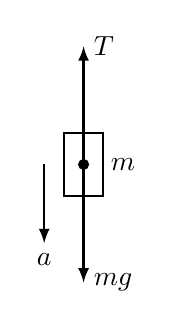
\begin{tikzpicture}[>=latex, thick]
        \draw (-.25, -.4) rectangle (.25, .4);
\draw [<->] (0,1.5)node [right]{$T$}--(0,-1.5)node [right]{$mg$};
\node at (.5,0){$m$};
\fill (0,0) circle(2pt);
\draw [->](-.5,0)--(-.5,-1)node [below]{$a$}; 
    \end{tikzpicture}
\qquad \qquad 
        \begin{tikzpicture}[>=latex, thick]
        \fill [pattern =north east lines](-1.5, 0) rectangle (1.5, -.2);
        \draw (-1.5,0)--(1.5,0);
\draw (-1,.25) rectangle (1,1.25);
\draw [->](-1,.75)--(-2,.75)node [above]{$T$};
\fill (-1,.75) circle(2pt);

\draw [->](.5,1.8)--node [above]{$a$}(-.5,1.8);
\node at (0,.75){$M$};

\draw [fill=white] (-.5, .25) circle (0.25);
\draw [fill=white] (.5, .25) circle (0.25);

    \end{tikzpicture}
    \caption{}
\end{figure}	

现在我们把装砂的砂桶和小车(连同砝码)分别作为研究对象,用隔离法分别分析它们的受力情况,并分别应用牛顿第二定律列出方程.它们的受力图如图10.11所示,它们的加速度的大小都是$a$,所以
\begin{align}
    \text{对小车}&\quad T=ma\\
    \text{对砂桶}&\quad mg-T=ma
\end{align}
从式(1)(2)消去$a$,解出$T$:
\begin{equation}
    T=\frac{M}{M+m}mg
\end{equation}

可见小车受到的拉力$T$并不等于砂和砂桶的总重量$mg$,而是比$mg$小一些,只有在砂和砂桶的总质量$m$远小于小车
和砝码的总质量$M$,即$m\ll M$时,才可以近似地取砂和砂桶的总重量为小车所受的拉力.在实验中,$m\ll M$这个条件通常都能满足,所以取砂和砂桶的总重量为小车受到的拉力,并认为只要砂和砂桶的总重量保持不变,小车受到的拉力也保持不变,这样做就包含了由于实验原理不完善而带来的系统误差.

\section{研究平抛物体的运动}

这个实验要描出平抛物体运动的轨迹,并求出平抛物体的初速度.
\begin{figure}[htp]\centering
    \includegraphics[scale=.45]{fig/10-13.png}
    \caption{}
    \end{figure}

实验装置如图10.12所示,用图钉把白纸钉在竖直的木板上,在木板的左上角固定着斜槽,固定斜槽时,要注意使它在末端$O$点的切线是水平的,在纸上把这个$O$点记下来,并利用重锤线在纸上通出通过$O$点的竖直线,把事先做好的有孔的纸卡片用手按在竖直木板上(图10.13),上下调整纸卡
片的位置,使槽上滚下的小球正好从纸卡片上的孔穿过.用铅笔在白纸上记下小球穿过这个孔时的位置.用同样的方法,记下小球穿过孔的一系列位置.实验时要注意,小球每次要在相同的高度从槽上滚下.
\begin{figure}[htp]
    \centering
    \includegraphics[scale=.45]{fig/10-12.png}
    \caption{}
\end{figure}

取下白纸,以$O$点为原点画出竖直向下的Y轴和水平向右的X轴,根据记下的小球穿过孔的一系列位置,用平滑的曲线画出小球做平抛运动的轨迹.

我们知道,平抛运动可以看作是两个分运动的合运动:一个是水平方向的匀速直线运动,速度等于平抛物体的初速度;另一个是竖直方向的自由落体运动,这样,测出曲线上某一点的坐标:$x$和$y$,已知$g$的数值,利用公式$y=\dfrac{1}{2}gt^2$和$x=vt$
就可以求出小球的水平分速度,这个分速度就是小球做平抛运动的初速度.

在曲线上选取几个不同的点,测出它们的坐标.用上述办法分别求出小球的初速度,最后算出平均值.

\section{验证向心力公式}
在这个实验里,我们来验证向心力公式$F=mr\omega^2$.
\begin{figure}[htp]\centering
    \includegraphics[scale=.45]{fig/10-14.png}
    \caption{}
    \end{figure}

图10.14是实验装置的示意图,在滚花部分用手指搓动转轴,使重锤$A$在水平面内做匀速圆周运动,并保持悬线竖直,弹簧水平拉长.这时,重锤做匀速圆周运动的向心力就是弹簧的拉力.(为什么?)

实验时,先称出重锤$A$的质量$m$,把它用线绳挂在水平横杆的一端,调整横杆和平衡体$B$的位置,使横杆两边大致平衡.量出重锤的臂长$r$,移动指示器$P$的位置,使它在重锰的正下方.在重锤和转轴之间挂上水平弹簧,因而重锤被拉向转轴.

然后,用手指搓动转轴,使重锤转动,并且保持重锤每转一周都从指示器的正上方通过.这时,可以看作重锤在做半
径为$r$的匀速圆周运动,测量重锤转100圈需要的时间,测
量三次,靠出其平均时间$t$.利用公式$\omega=200\pi/t$(自己推导这个公式)计算出$\omega$.将实验得到的$m$、$r$和$\omega$代入向心力公式,算出向心力$F$.

停止转动后,用测力计钩住重锤,把它水平拉到指示器的正上方,这时测力计测得的拉力$F'$就是重锤做半径为$r$的匀速圆周运动所需的向心力.

把上述的测量数据和计算结果填入自己设计的表中,比较用向心力公式得到的$F$和用测力计测得的$P$在误差范围是否相等.

分别改变重锤的质量$m$、半径$r$和弹簧的倔强系数,重做
上述实验,并比较$F$和$F'$.

\section{研究有固定转动轴物体的平衡条件}
在这个实验里,我们利用力矩盘来研究有同定转动轴物体的平衡条件.
\begin{figure}[htp]\centering
    \includegraphics[scale=.45]{fig/10-15.png}
    \caption{}
    \end{figure}

如图10.15所示,装好力矩盘,使它竖直地支在金属轴$O$上.在盘上任意选择四个位置,各插一根大头针,其中三根针上用细线分别悬挂不同个数的钩码,第四根针上用细线挂弹簧秤,弹簧秤的另一端挂在横杆的套环上.

当力矩盘在这四个力作用下处于平衡状态的时候,量出各个力的力臂,测量时要注意:某个力的力臂是这个力的作用线到轴的垂直距离,而不是它的作用点到轴的距离.

自己设计一个表格,把力和力臂的数值填入表里.在记录数据的时候,要弄清楚哪个作用力是使物体反时针转动,哪个作用力是使物体顺时针转动,以便确定力矩的正负.

改变大头针的位置和各个力的大小,再重做几次.

在你所做的几次实验里,各个力的力矩的代数和在实验误差范围内是否等于零?你的实验结论是什么?

作用在盘的四个力,有一个是弹簧秤的弹簧的弹力,而不是钩码的重力,这对做实验有什么好处?

\section{验证机械能守恒定律}
在这个实验型,我们来验证机械能守恒定律.

先来研究物体自由下落的情况,如果忽路空气的阻力,物体的机械能守恒,即重力势能的减少等于动能的增加,设物体的质量为$m$,下落高度为$h$时的速度为$v$,则有
\[\frac{1}{2}mv^2-mgh\]

现在按照图10.16所示的装置,用打点计时器来做实验.接通电源,松开纸带,让重物拖着纸带自由下落,纸带上打下一列小点.
\begin{figure}[htp]
    \centering
    \includegraphics[scale=1]{fig/10-16.pdf}
    \caption{}
\end{figure}

取下纸带,记下第一个点的位置$O$,在纸带上选取方便的5个连续点$A,B,C,D,E$.测出和邻两点间的距离
$s_1,s_2,s_3,s_4$.再用实验七的方法分别算出打点计时器在打$B,C,D$各点时,重物的下落速度
\[v_1=\frac{s_1+s_2}{2t},\quad v_2=\frac{s_2+s_3}{2t},\quad v_3=\frac{s_3+s_4}{2t},\qquad t=0.02{\rm s}\]
把测量和算出的数据填入自己设计的表格里.算出重物增加的动能
\[\frac{1}{2}mv_1^2, \quad \frac{1}{2}mv_2^2, \quad \frac{1}{2}mv_3^2\]
利用当地的$g$值算出相应减少的重力势能$mgh_1,mgh_2,mgh_3$.这里的$h_1,h_2,h_3$分别是打点计时器在打$B$、$C$、$D$各点时,重物下落的高
度,即$B$、$C$、$D$各点离第一个点$O$的距离.根据机械能守恒定律应当有:
\[mgh_1=\frac{1}{2}mv^2_1,\quad mgh_2=\frac{1}{2}mv^2_2,\quad mgh_3=\frac{1}{2}mv^2_3\]
你计算的结果如何?(这里并不需要知道动能和势能的具体数值,因此不需要测出重物的质量)

下面来研究物体在重力作用下沿斜面运动的情况,物体沿斜面运动时,斜面对物体的支持力不做功,如果忽略空气阻力和摩擦力,物体的机械能守恒,即物体的重力势能的减少等于动能的增加.

\begin{figure}[htp]
    \centering
    \includegraphics[scale=.45]{fig/10-17.png}
    \caption{}
\end{figure}

我们仍然用打点计时器来做这个实验,实验装置如图10.17所示,让小车拖着纸带沿斜面滑下,在纸带上打下一列
小点.象前面所讲的那样,记下纸带上第一个点的位置$O$,在纸带上选取5个连续点$A,B,C,D,E$.分别求出3个下滑速度
\[v_1=\frac{s_1+s_2}{2t},\quad v_2=\frac{s_2+s_3}{2t},\quad v_3=\frac{s_3+s_4}{2t}\]
测出斜面的长度$\ell$和高度$H$,计算出重物下落的相应高度
\[h_B=\frac{H}{\ell}d_B, \quad h_C=\frac{H}{\ell}d_C, \quad h_D=\frac{H}{\ell}d_D \]
这里的$d_B$、$d_C$、$d_D$分别是$B$、$C$、$D$各点离第一个点$O$的距离.把求得的数据填在自己设计的表格里,算出$\dfrac{1}{2}mv^2$和相应的$mgh$,看看它们是否相等.

比较上面两种情况,将会发现后一情况能量损失较大,这是什么原因?实验误差的主要来源是什么?你能提出什么办法来减小误差?

\section{研究弹性碰撞}
这个实验要研究弹性碰撞中动量守恒和动能守恒.实验
装置如图10.18所示,让一个小球从斜槽上滚下来,跟放在斜槽末端的另一个质量较小的球发生正碰,测出两球的质量以及它们碰撞前后的速度,就可以研究弹性碰撞中动量和动能是否守恒.
\begin{figure}[htp]
    \centering
    \includegraphics[scale=.5]{fig/10-18.png}
    \caption{}
\end{figure}

小球的质量可以用天平来测量,怎样测定两球碰撞前后的速度呢?实验时将斜槽固定在桌边,并注意使斜槽的末端点的切线是水平的,被碰小球支在小柱上,两球碰撞时一样高,碰撞前后的速度都是水平的.因此,两球碰撞前后的速度,可以利用我们学过的平抛运动的知识求出来.

做平抛运动的小球下落到地面,它们下落的高度相同,飞行时间也相同,这样,小球的水平速度与其飞出的水平距离成正比,如果用小球的飞行时间作时间单位,小球飞出的水平距离在数值上就等于它的水平速度.

为了记录小球飞出的水平距离,在地上铺一张白纸,白纸
上铺放复写纸,小球落在复写纸上,就在白纸上留下小球落地位置的痕迹,利用这个痕迹我们不难测出小球飞出的水平距离.

上面讲了实验装置和实验原理,现在我们做实验.

先不放上被碰小球,让入射小球从斜槽上某一高度滚下,重复10次,用尽可能小的圆把所有的小球落点图在里面,圆心$P$就是小球落点的平均位置(图10.19).
\begin{figure}[htp]
    \centering
    \includegraphics[scale=.5]{fig/10-19.png}
    \caption{}
\end{figure}

把被碰小球支在小柱上,让入射小球从同一高度滚下,使它们发生正碰.重复10次,用同样的办法标出入射小球的落点的平均位置$M$、被碰小球的落点的平均位置$N$.

现在来测量小球飞出的水平距离.

我们看到实验装置中有个重垂线,它的悬点正好在斜槽的末端点.在白纸上记下重垂线所指的位置$O$,它表示斜槽的末端点在纸上的垂直投影.不发生碰撞时入射小球飞出的水平距离应当从斜槽末端点在纸上的垂直投影算起,因此线段$OP$是不发生碰撞时入射小球飞出的水平距离,它在数值上等于入射小球碰擅前的速度$v_1$.

支持被碰小球的小柱和斜槽末端点的距离为$2r$,其中$r$是两个小球的半径,在直线$ON$上取线段$OO'=2r$,则$O'$点就是碰撞时被碰小球的球心在纸上的垂直投影,因此线段$O'N$ 是被被小球碰撞后飞出的水平距离,它在数值上等于被碰小球碰撞后的速度$v'_2$.

从图10.19可以看出,碰撞时入射小球的球心在斜槽末端点的上方,因此线段$OM$是入射小球碰撞后飞出的水平距离,它在数值上等于入射小球碰撞后的速度.

测量完毕,我们可以利用测量结果进行研究了.

先研究动量守恒,根据动量守恒定律应当有
\[m_1v_1=m_1v'_1+m_2v'_2 \]
因为$v_1, v'_1,v'_2$在数值上分别等于线段$OP$, $OM$, $O'N$的长度,
所以
\[m_1(OP)=m_1(OM)+m_2(O'N)\]
把测得的数据代入上式,看看等式是否成立.

再来研究动能守恒.在弹性碰撞中动能守恒,所以应当
有
\[\begin{split}
    \frac{1}{2}m_1v_1^2&=\frac{1}{2}m_1{v'_1}^2+\frac{1}{2}m_2{v'_2}^2\\
    m_1(OP)^2&=m_1(OM)^2+m_2(O'N)^2
\end{split}\]
把测得的数值代入上式,看看等式是否成立.

根据实验结果,总结弹性碰撞的规律.

做这个实验的时候,入射小球的质量$m_1$必须大于被碰小
球的质量$m_2$.你能利用所学知识来说明其中的道理吗?

在研究弹性碰撞中动能守恒时,也可以不用等式
\[m_1(OP)^2=m_1(OM)^2+m_2(O'N)^2\]
而把测得的数据代入等式$O'N-OM=OP$中,看看它是否成
立,就知道动能是否守恒.研究一下这个问题,说明道理,并
把你测得的数据代入后一等式,看看它是否成立.


\section{用冲击摆测弹丸的速度}
冲击摆是一个用细线悬挂
着的沙箱,弹丸击中沙箱时陷
入箱内,使沙箱摆至某一高度
(图10.20),利用这种装置可
以测出弹丸的速度.
\begin{figure}[htp]\centering
\begin{tikzpicture}[>=latex, scale=1.5]
        \fill [pattern=north east lines](-.5,0) rectangle (.5,0.25);
        \draw (-.5,0)--(.5,0);
\draw [rotate=30, dashed] (-.35, -3.5) rectangle (.35, -3);
\draw  (-.35, -3.5) rectangle (.35, -3);
\draw (0,0)--(-90:3);\draw[dashed] (0,0)--(-60:3);

\draw[fill=gray] (-2+1, 5.3-8.5) --(-1.7+1, 5.3-8.5) to [bend left=15] (-1.45+1, 5.2-8.5) to [bend left=15] (-1.7+1,5.1-8.5)--(-2+1,5.1-8.5)--(-2+1,5.3-8.5); 

\draw[rotate=30, fill=gray] (-2+1.7, 5.3-8.5) --(-1.7+1.7, 5.3-8.5) to [bend left=15] (-1.45+1.7, 5.2-8.5) to [bend left=15] (-1.7+1.7,5.1-8.5)--(-2+1.7,5.1-8.5)--(-2+1.7,5.3-8.5); 

\draw [dashed](0,-3.25)--(3,-3.25);
\draw [dashed](1.7,-2.8)--(3,-2.8);
\draw[<->](2.3,-3.25)--node[right]{$h$}(2.3,-2.8);
    \end{tikzpicture}
    \caption{}
    \end{figure}

先来讨论这种测弹丸速度
的方法.

设弹丸的质量为$m$,速度
为$v$,沙箱的质量为$M$.弹丸未
射入沙箱前,沙箱静止在平衡位置,弹丸和沙箱的总动量为
$mv$;弹丸击中沙箱后,弹丸和沙箱以相同的速度运动,设这个
速度为$v'$,它们的总动量为$(M+m)v'$.根据动量守恒定律
\begin{equation}
    mv=(M+m)v'
\end{equation}

弹丸和沙箱一起运动后,线的拉力不做功,只有重力做
功,机械能守恒.因此,它们在开始运动时的动能,在到达最
高位置时完全转化成重力势能.设摆动的最大高度为$h$,根
据机械能守恒定律
\begin{equation}
    \frac{1}{2}(M+m){v'}^2 =(M+m)gh
\end{equation}
即
\[v'=\sqrt{2gh}\]
代入(10.4)式后可得
\begin{equation}
v=\frac{M+m}{m}\sqrt{2gh}
\end{equation}

\begin{figure}[htp]
    \centering
    \includegraphics[scale=.4]{fig/10-21.png}
    \caption{}
\end{figure}

现在我们用图10.21所示的装置来做实验.这个装置主
要由冲击摆和弹簧枪组成,冲击摆的摆锤用四根线绳悬挂着,
线绳的长度可以调节.摆锤是中空的,弹丸射入摆锤后,被卡
在里面,不能反跳出来.弹簧枪用来发射弹丸.它有三档,能
够发射三种不同的弹丸速度.摆锤摆动时,推动着指针偏转.
这个指针可以停留在任一位置上,实验中根据指针停留的位
置就可以从刻度盘上读出摆锤摆动的最大角度.设摆锤摆动	
的最大角度为$\theta$、摆长为$\ell$,那么摆锤摆动的最大高度
\begin{equation}
    h=\ell(1-\cos\theta)
\end{equation}
这个公式,请同学们自己证明.

做实验时,要将实验装置水平放在桌子上.调节四根线
绳的长度,使弹丸恰好能射入摆锤内,并使摆锤摆动平稳,让
冲击摆在平衡位置静止.扳动弹簧枪的扳机,把弹丸射入摆
锤内.摆锤和弹丸一起摆动,并推动着指针偏转,摆锤在推
动指针偏转时,要克服摩擦力做功.因此实验时,应使指针先
停留在适当的高度,以减少能量的损耗.记下摆锤摆动的最
大角度$\theta$,测出悬线的长度,它就是摆长$\ell$,即可用公式(10.7)算
出最大高度 $h$,用天平分别测出弹丸的质量$m$和摆锤的质量
$M$,最后用公式(10.6)求出弹丸的速度.

用同样的方法,求出弹簧枪另外两档发射的弹丸速度.

\section{用单摆测定重力加速度}
我们知道,单摆在偏角很小时,它的周期公式是
\[T=2\pi\sqrt{\frac{\ell}{g}}  \]
如果测出单摆的摆长和周期,利用单摆周期公式使可以求出
当地的重力加速度$g$的数值.

选取一段1米左右的细线,让线的一端穿过小球的小孔,
然后打一个比小孔大一些的线结,这样就做成一个单摆.把
线的上端用铁夹固定在铁架台上,把铁架台放在实验桌边,使
铁夹伸到桌面以外,让摆球自由下垂.

用米尺量出悬线长$\ell'$,准确到毫米,为了测量方便,可以
用游标卡尺测量摆球的直径,然后算出摆球的半径$r$,也准确
到毫米.单摆的摆长是悬点到球心的距离,所以$\ell+r$就是摆
长.

把单摆从平衡位置拉开一个很小的角度(不超过5$^\circ$),然
后放开小球让它摆动,用秒表测出摆动30—50次的时间,计
算出平均摆动一次的时间,这个时间就是单摆的振动周期.

根据单摆的周期公式,计算出重力加速度.

变更摆长,重做几次实验,计算出每次实验的重力加速
度.最后,求出几次实验得到的重力加速度的平均值,即是本
地区的重力加速度.

设计一个表格,把测得的数据和计算结果填入表中.

利用实验中测得的数据还可以研究周期跟摆长的关系.
从单摆的周期公式知道,周期跟摆长的平方根成正比.算出
不同摆长下周期跟相应的摆长的平方根之比,看看这些比值
是否相等.

从单摆的周期公式知道,周期跟偏角的大小、摆球的质量
没有关系,用实验验证一下这个结论.


